\chapter{Hasil dan Analisis}

\section{Prelude: Pemilihan Training Data}

Perlu diperhatikan bahwa pada kasus ini, anomaly detection dikembangkan dengan pendekatan \emph{unsupervised learning}. Hal ini karena data \texttt{'machine status'} tidak mewakili apakah data berupa anomaly atau tidak.Ingat bahwa permasalahan yang ingin diselesaikan disini adalah mencari pola pada data yang mengindikasi penyebab kerusakan mesin. Hal ini berarti anomaly yang ingin dideteksi terjadi sebelum status mesin \texttt{BROKEN}. 

Data pada bulan 8 dipilih sebagai training data karena pada bulan tersebut tidak terjadi kerusakan mesin. Disini penulis berasumsi bahwa pada bulan 8 tidak terjadi anomali sama sekali pada data, karena tidak terjadi kerusakan mesin. Namun pada bulan lainnya, walau ada bagian data yang memiliki status mesin NORMAL, bisa saja sebenarnya sudah terjadi anomaly yang menyebabkan machine BROKEN pada hari-hari setelahnya.

\section{Hasil}
\subsection{LSTM Autoencoder}

Data dipisah menjadi dua bagian, yaitu data normal yang mengandung data dari status NORMAL dan data anomali yang berasal dari status selain NORMAL (BROKEN dan RECOVERY).

Kemudian data dibagi menjadi 3 dataset, yaitu train, validation, dan test. Data train dan validation diambil pada bulan ke-8 awal dan akhir masing-masing dan digunakan untuk training model, sedangkan data test diambil pada selain bulan ke-8 untuk memprediksi hasil anomali.

Proses training model LSTM Autoencoder dilakukan sebanyak 5 epoch yang memakan waktu sekitar 20 menit dengan menggunakan GPU (CUDA). Data train dan validation dibagi menjadi dua macam, yaitu dengan PCA dan tanpa PCA.

Kemudian dilakukan prediksi pada data test dari model yang telah dilakukan training sehingga dapat diperoleh nilai loss yang dihasilkan.

    \subsubsection{Dengan PCA}

    \begin{figure}[h]
        \centering
        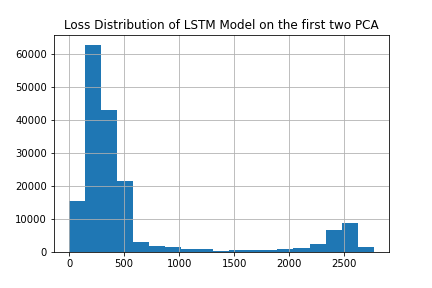
\includegraphics[width=0.6\textwidth]{resources/LSTM/LSTM_PCA_LossDist.png}
        \caption{Distribusi loss LSTM dengan PCA}
    \end{figure}

    Dengan menggunakan nilai threshold 500, diperoleh jumlah data anomali sebagai berikut.

    \begin{table}[h]
        \centering
        \begin{tabular}{|l|r|r|r|}
            \hline
            \multicolumn{1}{|c|}{\textbf{Jenis anomali}} & \multicolumn{1}{c|}{\textbf{Jumlah}} & \multicolumn{1}{c|}{\textbf{Total data}} & \multicolumn{1}{c|}{\textbf{Persentase (\%)}} \\ \hline
            Anomali pada data NORMAL                     & 33866                                & 160430                                   & 21                                       \\ \hline
            Anomali pada data selain NORMAL              & 2237                                 & 14454                                    & 15                                       \\ \hline
        \end{tabular}
    \end{table}

    Jumlah anomali pada data selain NORMAL tidak mencakup keseluruhan total data sehingga terdapat prediksi yang berada pada data dalam kondisi BROKEN atau RECOVERY.

    \subsubsection{Tanpa PCA}

    \begin{figure}[h]
        \centering
        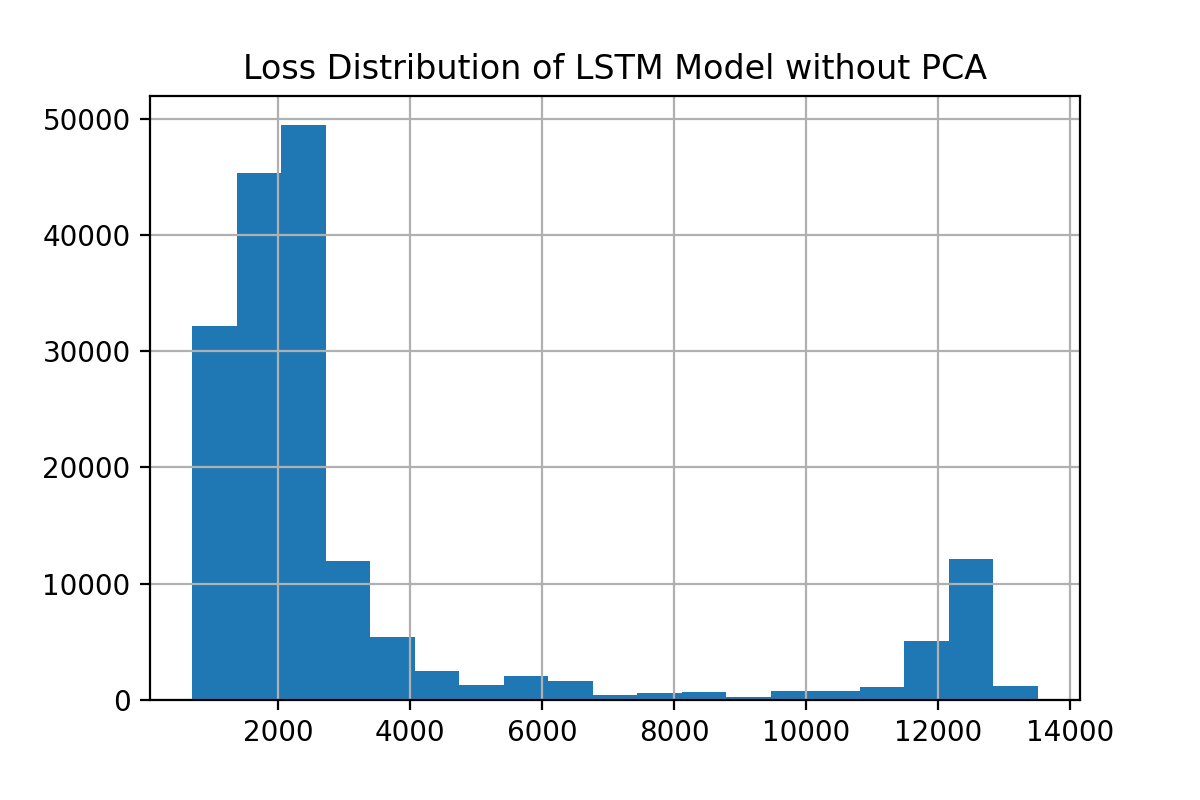
\includegraphics[width=0.6\textwidth]{resources/LSTM/LSTM_noPCA_LossDist.png}
        \caption{Distribusi loss LSTM tanpa PCA}
    \end{figure}

    Dengan menggunakan nilai threshold 3500, diperoleh jumlah data anomali sebagai berikut.

    \begin{table}[h]
        \centering
        \begin{tabular}{|l|r|r|r|}
            \hline
            \multicolumn{1}{|c|}{\textbf{Jenis anomali}} & \multicolumn{1}{c|}{\textbf{Jumlah}} & \multicolumn{1}{c|}{\textbf{Total data}} & \multicolumn{1}{c|}{\textbf{Persentase (\%)}} \\ \hline
            Anomali pada data NORMAL                     & 30182                                & 160430                                   & 19                                       \\ \hline
            Anomali pada data selain NORMAL              & 4979                                 & 14454                                    & 34                                       \\ \hline
        \end{tabular}
    \end{table}

    Terlihat bahwa jumlah anomali pada data NORMAL lebih sedikit 3\% dari analisis dengan PCA, Namun jumlah anomali pada data selain NORMAL juga meningkat hampir 2 kali lipat.

\subsection{Bayesian Probability}

Data dipisah menjadi training data dan test data. Tidak ada validation data disini, karena validation data digunakan untuk mencegah model overfitting pada training data. Namun karena model bayesian adalah distribusi probabilitas, maka validation data akan menggeser kontur probabilitas dari overfitting pada training data menjadi tepat fit pada training dan validation data sekaligus. Jadi hasilnya tidak akan ada bedanya jika model dilatih pada training dan validation data yang digabungkan. Karena itu, validation data sudah digabungkan kedalam training data, yaitu data pada bulan 8.

Hasil prediksi model Bayesian pada test data menghasilkan distribusi probabilitas data merupakan data normal sebagai berikut.
\begin{figure}[h]
    \centering
    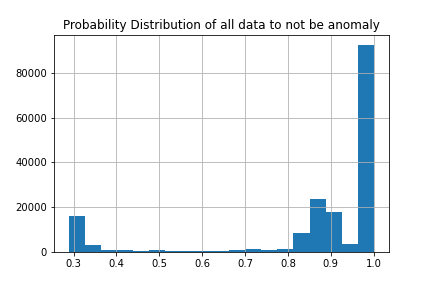
\includegraphics[width=0.8\textwidth]{resources/Bayes/Bayes_ProbDist.png}
    \caption{Prediksi Probabilitas bukan Anomali}
\end{figure}
Kemudian probabilitas tidak terjadi anomali dan terjadi anomali pada tiap waktu sebagai berikut.
\begin{figure}[h]
    %\centering
    \centerline{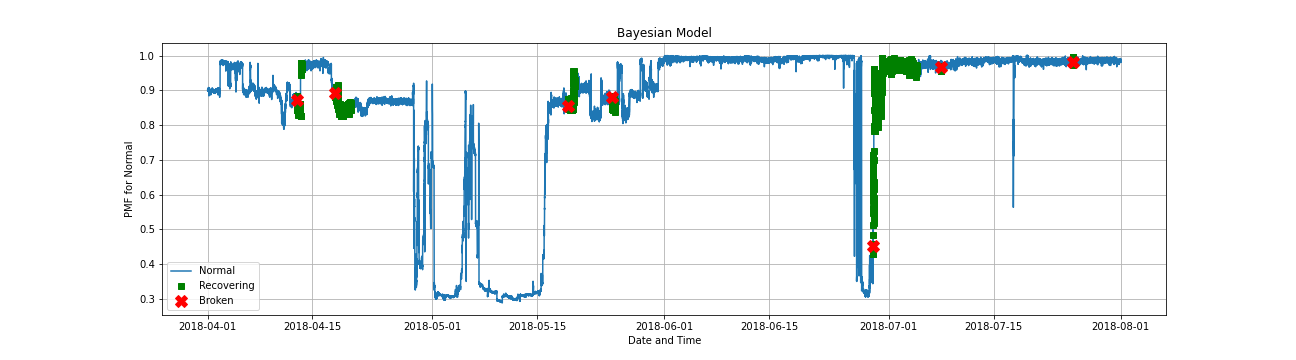
\includegraphics[width=1.4\textwidth]{resources/Bayes/Bayes_normal_PMF.png}}
    \caption{Prediksi Probabilitas bukan Anomali}
\end{figure}
\begin{figure}[h]
    %\centering
    \centerline{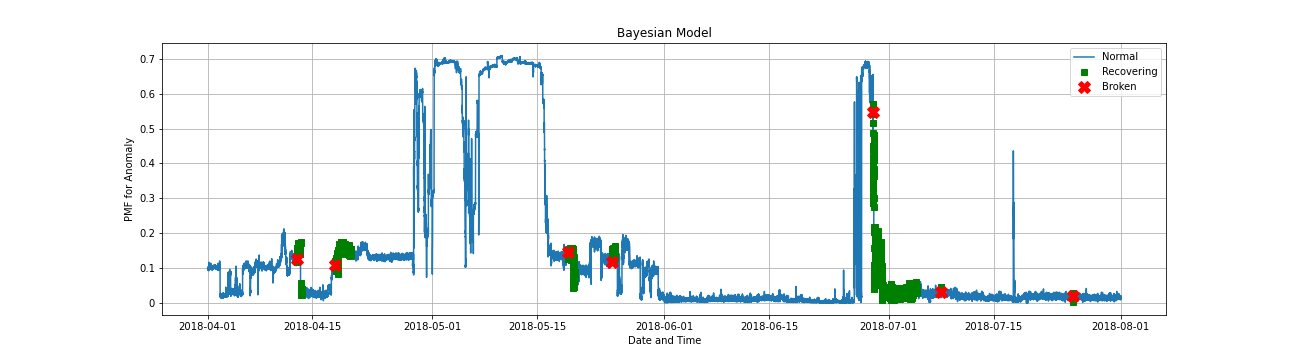
\includegraphics[width=1.4\textwidth]{resources/Bayes/Bayes_anomaly_PMF.png}}
    \caption{Prediksi Probabilitas terjadi Anomali}
\end{figure}
Dengan menetapkan nilai threshold sebesar 0.85, ini berarti jika probabilitas suatu data merupakan data normal dibawah 0.85 sudah ditetapkan sebagai data yang likely merupakan anomaly. Diperoleh jumlah data anomali sebagai berikut.
\begin{table}[h]
    \centering
    \begin{tabular}{|l|r|r|r|}
        \hline
        \multicolumn{1}{|c|}{\textbf{Jenis anomali}} & \multicolumn{1}{c|}{\textbf{Jumlah}} & \multicolumn{1}{c|}{\textbf{Total data}} & \multicolumn{1}{c|}{\textbf{Persentase (\%)}} \\ \hline
        Anomali pada data NORMAL                     & 34527                                & 160430                                   & 22                                       \\ \hline
        Anomali pada data selain NORMAL              & 2567                                 & 14454                                    & 18                                       \\ \hline
    \end{tabular}
\end{table}

\section{Analisis}
\subsection{Komparasi Kecepatan Proses}
Kecepatan proses yang diukur adalah durasi waktu yang dibutuhkan untuk model training. Didapatkan hasil berikut.

\begin{table}[h]
    \centering
    \begin{tabular}{|l|r|l|}
        \hline
        \multicolumn{1}{|c}{\textbf{Model}} & \multicolumn{1}{|c|}{\textbf{Durasi Model Training}} & \multicolumn{1}{c|}{\textbf{Keterangan}} \\ \hline
        Interquartile Range (IQR)   &        1s 100ms 176$\mu$s    & Acuan \\
        K-Means Clustering          &       46s 063ms 282$\mu$s    & Acuan \\
        Isolation Forest            &       15s 139ms 811$\mu$s    & Acuan \\
        Bayesian Probability        &       15s 031ms 475$\mu$s    & Kembangan \\
        LSTM Autoencoder dengan PCA &   18m 02s 607ms 847$\mu$s    & Kembangan \\
        LSTM Autoencoder tanpa PCA  &   39m 20s 885ms 569$\mu$s    & Kembangan \\
        \hline
    \end{tabular}
\end{table}

Terlihat bahwa durasi model training cukup cepat, kecuali untuk model LSTM Autoencoder. Hal ini karena LSTM Autoencoder memiliki basis Neural Network yang mempunyai multilayer. Dalam model yang penulis kembangkan, total layer sebanyak 128 lapis, yang membuat proses komputasi cukup ekstensif walau sudah dibantu dengan menggunakan driver CUDA.

Model IQR dan Bayesian membutuhkan durasi yang cukup sedikit. Hal ini karena model dilatih dengan perhitungan statistik yang sederhana secara komputasi. Model IQR hanya perlu menghitung tiap data terhadap range antar quartil atas dan quartil bawah. Kemudian model Bayesian sudah menggunakan penyederhanaan matematik secara analitik yang cukup panjang, sehingga iterasi numerik yang perlu dilakukan tidak terlalu kompleks. Hal ini juga dibantu dengan scale down data input pada model Bayesian. Walaupun model Bayesian yang menggunakan matematik yang jauh lebih rumit dibandingkan IQR membuat durasi training 15x lebih lama.

Model K-Means Clustering dan Isolation Forest memakan durasi yang kecil karena pendekatan yang dilakukan adalah menganggap data hanya terbagi antara 2 kluster saja, yaitu kluster normal dan anomaly. Apabila asumsi kluster lebih dari 2 mungkin akan memakan waktu lebih lama, namun ini sudah bukan lagi Anomaly Detection melainkan Clustering Data.

\subsection{Perbandingan Prediksi Anomali}
Ketiga model memiliki ....

\begin{figure}[h]
    %\centering
    \centerline{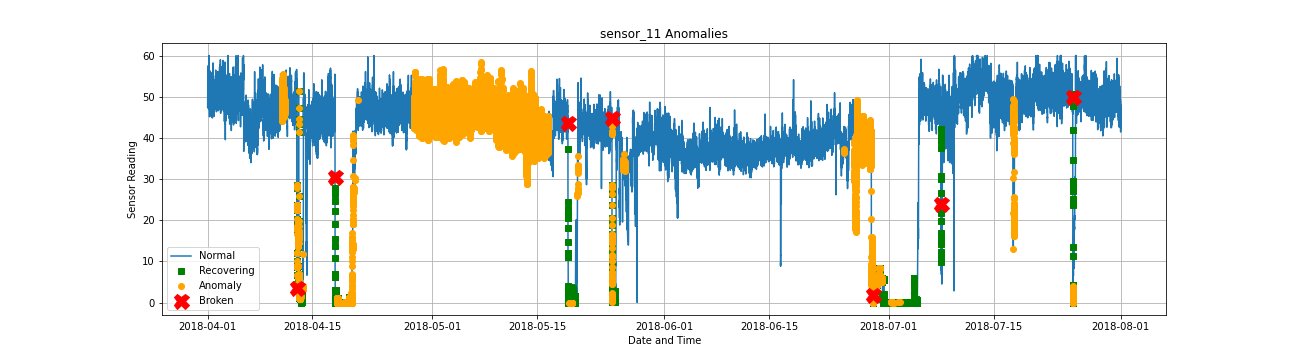
\includegraphics[width=1.4\textwidth]{resources/LSTM/LSTM_noPCA_sensor_11.png}}
    \caption{Hasil deteksi anomali model LSTM tanpa PCA}
\end{figure}
\begin{figure}[h]
    %\centering
    \centerline{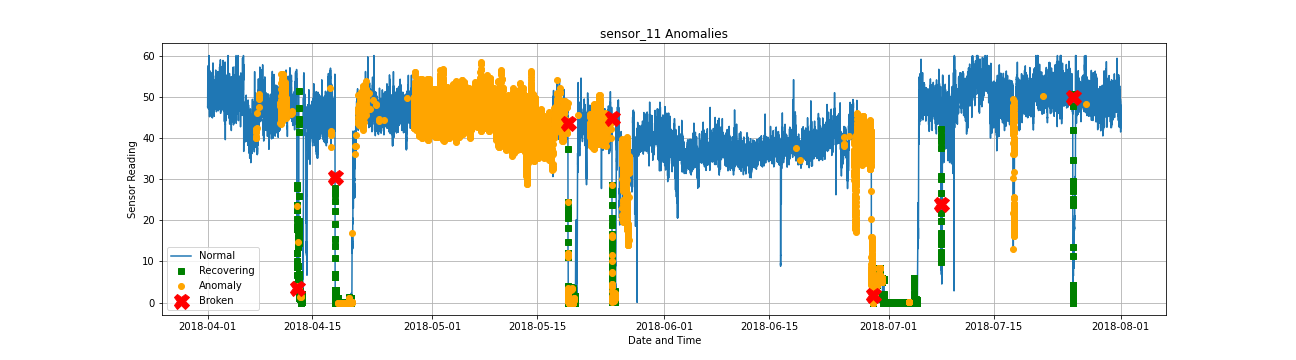
\includegraphics[width=1.4\textwidth]{resources/LSTM/LSTM_PCA_sensor_11.png}}
    \caption{Hasil deteksi anomali model LSTM dengan PCA}
\end{figure}
\begin{figure}[h]
    %\centering
    \centerline{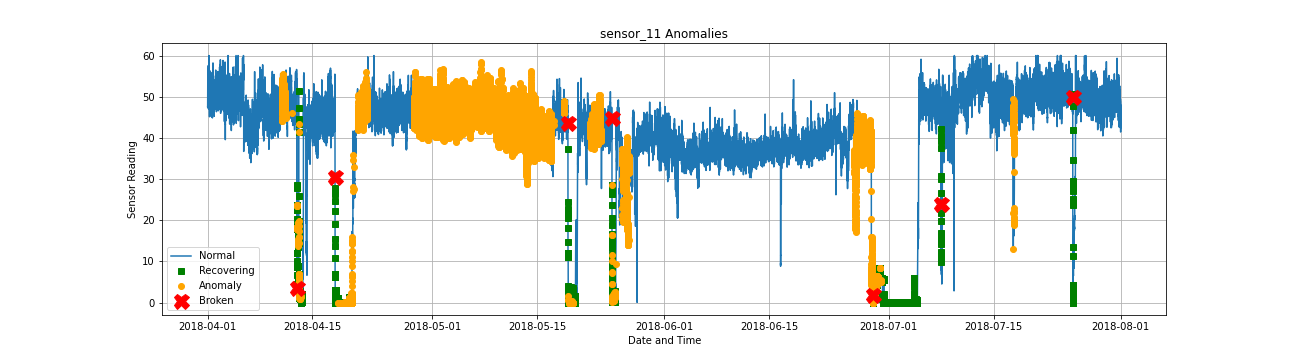
\includegraphics[width=1.4\textwidth]{resources/Bayes/Bayes_sensor_11.png}}
    \caption{Hasil deteksi anomali model Bayesian}
\end{figure}
